\chapter[Introdução]{Introdução}

Este capítulo apresenta a contextualização, o problema de pesquisa, a justificativa,
os objetivos, a metodologia de pesquisa utilizada e a organização deste trabalho.

\section[Contextualização]{Contextualização}

O processo de ensino aprendizagem tem sofrido grandes mudanças desde as transformações cientificas na segunda metade do século XX. O surgimento de pesquisas sobre o aprendizado e novas formas de ensino se deu naturalmente, motivado pelo desenvolvimento do pensamento sistêmico e as novas tendências de produção industrial enxuta, que exigiam trabalhos científicos e novas propostas para o sistema educacional. Já que a forma programada e linear de ensino utilizado após a primeira revolução industrial não se adequava mais às necessidades contemporâneas de raciocínio e tomadas de decisão requeridas do profissional intelectual \cite{oliveira2009, frigotto1989}.

Por volta de 1950 aconteceram as primeiras tentativas de integrar a computação ao processo de ensino, nesse período surgiram os primeiros sistemas direcionados para a educação mediada por computador, foram os chamados Instrução Assistida por Computador, ou \textit{Computer Assisted Instruction} (CAI). Esses sistemas tinham como pressuposto teórico o Behaviorismo, em que a instrução era feita de forma linear e subdividida em diversos módulos sequenciais. Ou seja, a instrução era baseada em uma modelagem de estímulos previamente definidos \cite{giraffa1995,vicari2003}.

Com a popularização da internet, por volta de 1990, surgiram os primeiros sistemas educativos para a web. Com base em teorias de hipermídias adaptativas \cite{brusilovsky1996} e de tutoria inteligente \cite{brusilovsky1994}, foram criados novos ambientes educacionais adaptativos e inteligentes que atuavam segundo modelos de usuário, traçados de acordo com o uso do sistema.

Nesse mesmo período apareceram as primeiras pesquisas em sistemas de vídeos interativos que, mesmo com o uso de vídeo cassete e um monitor, permitiam maior controle e interação do aprendiz com o material de aprendizado, o que corrobora para uma aprendizagem mais efetiva \cite{zhang2005}. Na época, foi possível verificar que a atividade era promissora mesmo na fase inicial de aplicação \cite{gaudreau1984}.

Já nos trabalhos mais recentes, há uma tendência para a utilização de sistemas tutores inteligentes combinados com as teorias de hipermídias adaptativas para uma melhor aprendizagem \cite{fragelli2010}. Fragelli discorre sobre uma nova abordagem para quantização de redes hipermídia que leva em consideração apenas as informações dos nodos, a Quantização de Redes por Nodos (QRN), e integra as teorias de hipermídias adaptativas, sistemas tutores inteligentes e objetos de aprendizagem (OA), que no caso específico deste trabalho, se configuram como vídeos interativos.

\section[Problema de Pesquisa]{Problema de Pesquisa}

Com base no contexto apresentado, este trabalho pretende verificar se é possível desenvolver uma navegação global adaptativa para um sistema \textit{web} de vídeos interativos utilizando a Quantização de Redes por Nodos.

\section[Justificativa]{Justificativa}

Apesar dos esforços realizados no desenvolvimento de sistemas inteligentes e adaptativos no processo de ensino, poucos foram os trabalhos que se preocuparam com a implantação e manutenção prática da tecnologia proposta, o que reforça a afirmação de que as linhas de pesquisa estão mais voltadas para o campo técnico do que para o âmbito da aprendizagem. Além disso, a QRN ainda não possui validação em um ambiente real de uso, sendo avaliada por especialistas na área com análises em diferentes redes hipermídias e com diferentes perfis de usuário \cite{fragelli2010}.

Outro fator a ser analisado é que os ambientes virtuais de aprendizagem exigem um grande número de OAs para serem efetivos, já que para alcançar o público de estudantes, tem-se a necessidade de produzir materiais mais elaborados e complexos segundo as diferentes necessidades cognitivas e perfis dos usuários. Para um professor-autor, essa característica desmotiva a produção dos materiais e corrobora a para a inutilização do sistema \cite{fragelli2010}. Dessa forma, seria uma boa medida se o sistema proposto contemplasse mecanismos facilitadores para a produção de recursos educacionais.

Ademais, segundo a Sinopse de Educação Superior publicada pelo Instituto Nacional de Estudos e Pesquisas Educacionais (INEP), o índice de desistência dos cursos na área de Engenharia, Produção e Construção nas instituições públicas chega a mais de 90\% dos matriculados (fig.  \ref{fig:matriculados}), o que indica uma grande desmotivação por parte dos alunos que pode ser explicada, dentre outros fatores, pelo alto nível de reprovações e pelo desnível entre os estudantes \cite{silva2005}.

\begin{figure}
	\begin{subfigure}{.5\textwidth}
  		\centering
  		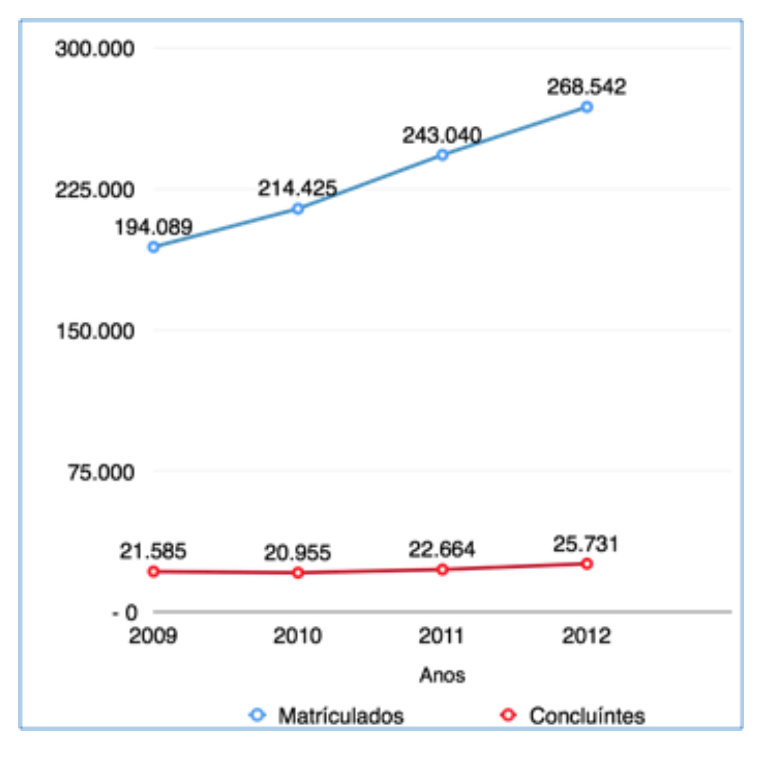
\includegraphics[width=.9\linewidth]{figuras/matriculados1.eps}
  		\caption{total de matriculados e concluintes.}
  		\label{fig:submat1}
	\end{subfigure}%
	\begin{subfigure}{.5\textwidth}
  		\centering
  		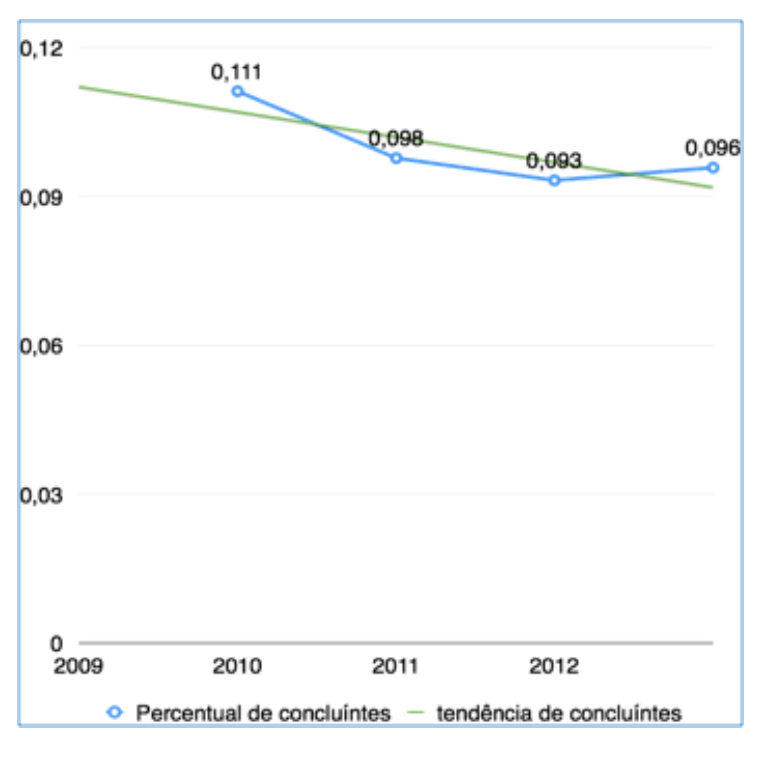
\includegraphics[width=.9\linewidth]{figuras/matriculados2.eps}
  		\caption{percentual de concluintes.}
  		\label{fig:submat2}
	\end{subfigure}
	\caption{Relação entre matriculados e concluintes em cursos de engenharia e construção
	(dados obtidos do INEP com a grande área Engenharia, Construção e Produção).}
	\label{fig:matriculados}
\end{figure}

Com base nesses fatores, o professor tem que alcançar um equilíbrio entre o mínimo e o razoável a ser ensinado, o que dificulta o aprofundamento em conteúdos mais elaborados e desafiadores, tornando frustrante o papel de educador, refletido em aulas monótonas e clássicas para um grupo de estudantes que vive o dinamismo tecnológico \cite{fragelli2010}.

Dessa forma, é necessário desenvolver sistemas de ensino que possibilitem uma aprendizagem adaptativa, contudo, é também importante motivar os professores a fazerem parte do processo de construção dos materiais que alimentam tais sistemas.

\section[Objetivos]{Objetivos}

O objetivo geral deste trabalho é desenvolver um sistema de vídeos educacionais interativos com navegação global adaptativa utilizando a QRN. Para tal, tem-se os seguintes objetivos específicos:
\begin{itemize}
  	\item Desenvolver um módulo de autoria de vídeos interativos que permita a criação dos objetos de aprendizagem, de modo a incentivar professores a construírem esses materiais.
  	\item Desenvolver um módulo de visualização dos vídeos interativos que adapte o conteúdo para os diferentes perfis de estudantes.
  	\item Desenvolver um mecanismo de navegação global adaptativa com a QRN para garantir a adaptação da navegação para diferentes perfis de estudantes.
\end{itemize}

\section[Metodologia]{Metodologia}
Levando em consideração os objetivos deste TCC, é utilizada a pesquisa exploratória com o intuito de compreender as linhas de pesquisa relacionadas aos sistemas inteligentes e adaptativos para o ensino, tendo como base os estudos em QRN, Sistemas de Hipermídias Adaptativas (SHA) e Vídeos Interativos para o desenvolvimento do sistema proposto.

Tendo isso em mente, e considerando também o âmbito da engenharia de software, o processo de desenvolvimento deste trabalho está fundamentado nas metodologias ágeis, mais especificamente as práticas do \textit{Scrum}. Já em relação ao desenvolvimento do sistema, são utilizados os paradigmas de programação Orientado a Objetos e o estilo arquitetural MVC.

Inicialmente, foram identificados os artigos científicos, dados informativos sobre os cursos de engenharia e possíveis tecnologias que se alinhem ao propósito deste trabalho, possibilitando um maior conhecimento dos domínios de ensino assistido por computador e de engenharia de software aplicada a sistemas \textit{web}.

O próximo passo foi definir o escopo do trabalho, levando em consideração as dimensões das áreas de pesquisa relacionadas ao ensino assistido por computador, e ao tempo disponível para o desenvolvimento. Além de serem definidas e estudadas também as tecnologias mais adequadas segundo as características do sistema.

Em paralelo a essas atividades, foi feito o refinamento da proposta para melhor se alinhar aos conceitos estudados no referencial teórico e foi feita a documentação do trabalho realizado para permitir, por fim, a escrita deste TCC e o desenvolvimento do sistema.

\section[Organização do Trabalho]{Organização do Trabalho}

Este trabalho está subdividido em cinco capítulos. No capítulo 2 é apresentado o referencial teórico utilizado nesta pesquisa, contendo um subtópico sobre os estilos de aprendizagem estudados para a proposta das redes hipermídias; posteriormente, um subtópico sobre os Princípios do Aprendizado Multimídia, exemplificando as heurísticas aplicadas na modelagem dos vídeos e como elas interferem no processo de ensino e aprendizagem; outro subtópico sobre Sistemas de Hipermídias Adaptativas e um subtópico sobre a QRN e as teorias que a fundamentam. É apresentado também o contexto da engenharia de software, com subtópicos sobre arquitetura de software, testes e  metodologia \textit{Scrum}.

No capítulo 3 é apresentado o desenvolvimento deste TCC, a modelagem do domínio do sistema, a arquitetura proposta e os módulos de autoria de materiais e de visualização adaptativa, bem como uma visão geral das estratégias de teste e desenvolvimento utilizadas na contrução do software.

O capítulo 4 discorre sobre as considerações a que se chegou com este estudo, o estado atual do desenvolvimento e as perspectivas de trabalhos posteriores.
